\documentclass[11pt]{beamer}
\usetheme{Boadilla}

\usepackage[utf8]{inputenc}
\usepackage[T1]{fontenc}
\usepackage{amsmath}
\usepackage{amsfonts}
\usepackage{amssymb}
\usepackage{graphicx}
\usepackage[scaled=0.85]{beramono}
\usepackage{listings}
\lstset{language=C++,
	columns=fullflexible,
	basicstyle=\ttfamily,
	tabsize=4,
} 
\usepackage[english]{babel}

\graphicspath{
	{\string~/Code/networkit/egosplit/plots/}
}


\begin{document}
	\author{Armin Wiebigke}
	\title{Ego-Splitting Framework}
	%\subtitle{}
	%\logo{}
	%\institute{}
	%\date{}
	%\subject{}
	%\setbeamercovered{transparent}
	%\setbeamertemplate{navigation symbols}{}
	\begin{frame}[plain]
	\maketitle
\end{frame}

\begin{frame}{Idea}
\begin{itemize}
	\item Overlapping community detection
	%\item Each node can be part of multiple communities
	\item Reduce problem to non-overlapping communities (partition)
	\begin{itemize}
		\item Many established algorithms
	\end{itemize}
	\item Ego-net of node \textit{u}: Subgraph induced by the neighbors of \textit{u}
	\item Two partition algorithms: local and global
\end{itemize}
\end{frame}


\begin{frame}{The Framework}
\begin{itemize}
	 \item For each node: Use the local clustering algorithm to partition the ego-net
	 \item Create persona graph:
	 \begin{itemize}
	 	\item Create a persona for each partition
	 	\item Add edges between personas
	 \end{itemize}
	 \item Use the global clustering algorithm on the persona graph
	 \begin{itemize}
	 	\item each partition equals a community
	 \end{itemize}
	 \item For each node: Collect communities from all personas
\end{itemize}
\end{frame}

\begin{frame}{Problems}
	\begin{itemize}
		\item local partitioning is critical
		\item number of Communities $\leq$ number of Personas
		\item Triangle with two nodes in community and one outside $\Rightarrow$ outside node is included in community by global partition algorithm 
	\end{itemize}
\end{frame}

\begin{frame}{Possible Improvements}
	\begin{itemize}
		\item Clean-up at the end (OSLOM)
		\item Connect personas of one node with additional edges
	\end{itemize}
\end{frame}

\begin{frame}{Plots}
	\centering
	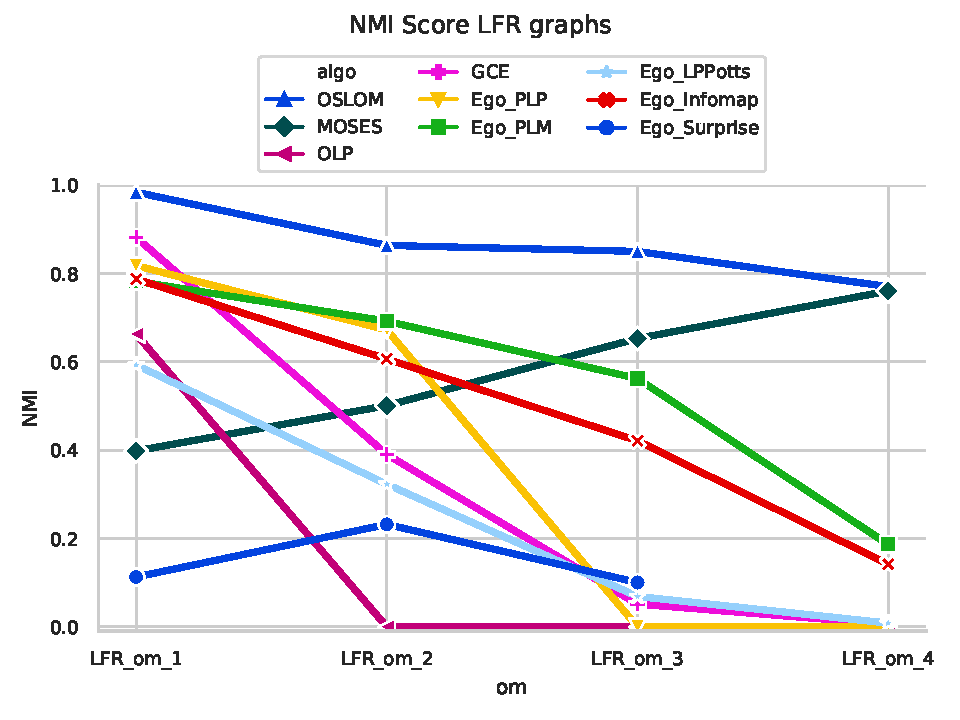
\includegraphics[width=0.8\linewidth]{metrics/NMI_score_LFR_om.pdf}
\end{frame}
\end{document}